% !TeX spellcheck = de_DE
\documentclass[a4paper,11pt]{ctexart}

\usepackage{setspace}
\usepackage{titlesec}
\usepackage{titletoc}
\usepackage[shortlabels]{enumitem}
\usepackage[hmargin=1.25in,vmargin=1in]{geometry}
\usepackage{amsmath}
\usepackage{amssymb}
\usepackage{indentfirst}
\usepackage[colorlinks,linkcolor=blue,anchorcolor=blue,citecolor=green]{hyperref}
\usepackage{tikz}
\usetikzlibrary{arrows.meta}
\usetikzlibrary{bending}
\usetikzlibrary{calc}
\usetikzlibrary{positioning}
\usetikzlibrary{math}
\usetikzlibrary{shapes.symbols}
\usetikzlibrary{shapes.geometric}
\usetikzlibrary{shapes.arrows}
\usepackage[american inductors]{circuitikz}
\usepackage{booktabs}
\usepackage{array}
\usepackage{multirow}
\usepackage{upgreek}
\usepackage{xfrac}
\usepackage{subfig}
\usepackage{float}
\usepackage{placeins}
\usepackage{url}
\usepackage{lscape}
\usepackage{rotating}
\usepackage{graphicx}
\graphicspath{{screen/}}
\usepackage{pythonhighlight}

\renewcommand\theequation{\arabic{equation}}
\renewcommand{\contentsname}{}
\renewcommand\arraystretch{1.5}

\newcommand{\kV}{\,\text{kV}}
\newcommand{\V}{\,\text{V}}
\newcommand{\Ohm}{\,\Omega}
\newcommand{\MOhm}{\,M\Omega}
\renewcommand{\H}{\,\text{H}}
\newcommand{\s}{\,\text{s}}
\newcommand{\kA}{\,\text{kA}}
\newcommand{\A}{\,\text{A}}
\newcommand{\MW}{\,\text{MW}}
\newcommand{\W}{\,\text{W}}
\newcommand{\MVar}{\,\text{MVar}}
\newcommand{\MVA}{\,\text{MVA}}
\renewcommand{\S}{\,\text{S}}
\newcommand{\km}{\,\text{km}}
\newcommand{\diff}{\text{d}}
\newcommand{\Hz}{\,\text{Hz}}
\newcommand{\kHz}{\,\text{kHz}}
\renewcommand{\j}{\text{j}}
\newcommand{\ssum}{\scriptscriptstyle \sum}
\newcommand{\dsp}{dsPIC33FJ32MC204}
%\renewcommand{\omega}{\upomega}

\newcommand{\du}[1]
{
	#1^{\circ}
}
\newcommand{\ang}[1]
{
	\angle#1^{\circ}
}

\newcommand{\bfem}[1]
{
	\em\bfseries#1\normalfont
}

\newcommand{\subpar}
{
	\par
	\hangafter = 0
	\setlength{\hangindent}{1em}
}

\newcommand{\subsubpar}
{
	\par
	\hangafter = 0
	\setlength{\hangindent}{2em}
}
\newcommand{\subsubsubpar}
{
	\par
	\hangafter = 0
	\setlength{\hangindent}{3em}
}



\newenvironment{shrinkeq}[2]
{
	\bgroup
	\addtolength\abovedisplayshortskip{#1}
	\addtolength\abovedisplayskip{#1}
	\addtolength\belowdisplayshortskip{#2}
	\addtolength\belowdisplayskip{#2}
}
{
	\egroup
	\ignorespacesafterend
}

\setcounter{secnumdepth}{4}

\title
{
	\linespread{1.5} \zihao{4}
	高压数字测量系统课程设计 \\ 
	\zihao{2}
	开题报告
}
\author
{
	谢弘洋
}
\date{}

\begin{document}
	\pagestyle{plain}

\begin{figure}[t]
	\setlength{\abovecaptionskip}{-10mm}
	\setlength{\belowcaptionskip}{-60mm}
	\centering
	
\includegraphics[scale=0.4]{page1.png}
\end{figure}

\begin{center}
	\zihao{-2}
	电\,气\,传\,动\,综\,合\,实\,验 \\
	\vspace{0.7em}
	
	\zihao{1}
	实\hspace{0.5em} 验\hspace{0.5em} 报\hspace{0.5em} 告\\
	\vspace{3em}
		
	\zihao{-3}
	\hspace{2em}姓名\hspace{1em} \underline{\hspace{4em}谢弘洋\hspace{4em}}\\
	\vspace{1em}
	\hspace{2em}学号\hspace{1em} \underline{\hspace{2.75em}515021910641\hspace{2.75em}}\\
	\vspace{1em}
	
	\vspace{6em}
	\today
\end{center}
\newpage
\begin{spacing}{1.5}
	\tableofcontents
\end{spacing}

\titleformat{\section}{\Large\bfseries\raggedright}{实验\chinese{section}}{10pt}{}
\titlespacing{\section}{0pt}{10pt}{5pt}
\titleformat{\subsection}{\bfseries\zihao{-4}}{\arabic{subsection}.}{5pt}{}
\titlespacing{\subsection}{1em}{2pt}{3pt}
\titleformat{\subsubsection}{\bfseries\normalsize}{\arabic{subsection}.\arabic{subsubsection}}{5pt}{}
\titlespacing{\subsubsection}{2em}{1pt}{0pt}
\titleformat{\paragraph}{\bfseries\normalsize}{}{0pt}{}
\titlespacing{\paragraph}{2em}{1pt}{0pt}

\newpage
\begin{spacing}{1.5}

\zihao{-4}


\section{BLDC开环控制}
\subsection{实验目标}
\begin{enumerate}[a.,topsep=0pt]
	\setlength{\itemsep}{-0.25\baselineskip}
	\item 编写程序,实现BLDC无刷电机的启动、运行与停止。
	\item 通过开发套件上的两个按钮外设,实现电机启动、停止和转动方向的控制。
	\item 熟悉实验开发套件的基本配置和使用方式,熟悉软件编写与调试工具的使用。
\end{enumerate}
\subsection{实验原理}
\subsubsection{BLDC无刷直流电机的运行}
\par
不同于有刷直流电机,无刷直流电机(Brushless DC Motor)最大的特点在于其转子由永磁体构成,因此不再需要外界通以电流来产生转子磁场,也就克服了传统直流电机转子需要换向器与电刷从而带来的一系列寿命、噪声上的问题。同时,定子也相应地由三相对称分布的绕组组成,当每个绕组上通以正负电流时,可以产生对应方向上的正负磁场。通常,BLDC的定子绕组采用两两通电方式,总共能够产生六种磁场方向的组合(如图\ref{figure:定子磁场组合}所示)。
\begin{figure}[h]
	\centering
	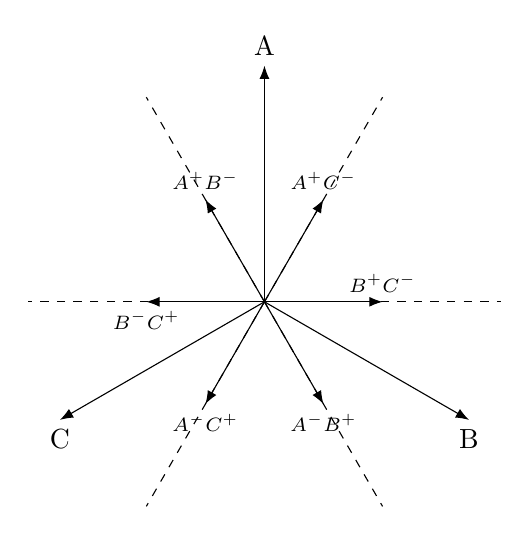
\begin{tikzpicture}[dummynode/.style={outer sep=-1,inner sep=-1}]
	\def\axe{3};
	\def\B{1.5};
	\draw [-Latex] (0,0) -- ++(90:\axe) node(A)[above]{A};
	\draw [-Latex] (0,0) -- ++(-30:\axe) node(B)[below]{B};
	\draw [-Latex] (0,0) -- ++(210:\axe) node(C)[below]{C};
	\draw [-Latex] (0,0) -- ++(0:\B) node(BPCM)[above]{$\scriptstyle B^{+}C^{-}$}; 
	\draw [-Latex] (0,0) -- ++(60:\B) node(APCM)[above]{$\scriptstyle A^{+}C^{-}$};
	\draw [-Latex] (0,0) -- ++(120:\B) node(APBM)[above]{$\scriptstyle A^{+}B^{-}$};
	\draw [-Latex] (0,0) -- ++(180:\B) node(BMCP)[below]{$\scriptstyle B^{-}C^{+}$};
	\draw [-Latex] (0,0) -- ++(240:\B) node(AMCP)[below]{$\scriptstyle A^{-}C^{+}$};
	\draw [-Latex] (0,0) -- ++(300:\B) node(AMBP)[below]{$\scriptstyle A^{-}B^{+}$};
	
	\foreach \t in {0,60,...,300}
		\draw [dashed] (0,0) -- ++(\t:\axe);
	\end{tikzpicture}
 	\caption{定子绕组两两通电产生的磁场矢量组合}\label{figure:定子磁场组合}
\end{figure}
\par
当定子磁场与转子磁场有一夹角时,就会产生磁场力矩,使两者有相互接近的趋势。而根据毕奥-萨法尔定律,磁场力与两个磁矢量之间夹角的正弦值成正比,因此当定子磁场方向与转子磁场方向垂直时,能够在相同的磁场大小(即定子绕组电流)下得到最大的力矩,提高电机的负载能力和效率。由此,可以按照这一准则将空间角度分为六个扇区,当转子磁场方向落在对应扇区时,即为对应的两个定子绕组同上对应方向的电流,产生与转子磁场方向正交的定子磁场,拖动转子旋转,如图\ref{figure:扇区划分}所示。
\begin{figure}[h]
	\centering
	\begin{tikzpicture}[dummynode/.style={outer sep=-1,inner sep=-1}]
	\def\axe{3};
	\def\B{1.5};
	\draw [-Latex] (0,0)node[dummynode](O1){} -- ++(90:\axe) node(A)[above]{A};
	\draw [-Latex] (O1) -- ++(-30:\axe) node(B)[below]{B};
	\draw [-Latex] (O1) -- ++(210:\axe) node(C)[below]{C};
	
	\foreach \t in {0,60,...,300}
		\draw [dashed] (O1) -- ++(\t:\axe);
	\draw (O1)++(270:\B) node(BPCM){$\scriptstyle B^{+}C^{-}$}; 
	\draw (O1)++(330:\B) node(APCM){$\scriptstyle A^{+}C^{-}$};
	\draw (O1)++(30:\B) node(APBM){$\scriptstyle A^{+}B^{-}$};
	\draw (O1)++(90:\B) node(BMCP){$\scriptstyle B^{-}C^{+}$};
	\draw (O1)++(150:\B) node(AMCP){$\scriptstyle A^{-}C^{+}$};
	\draw (O1)++(210:\B) node(AMBP){$\scriptstyle A^{-}B^{+}$};
	\draw (O1)++(0,-\axe) node{逆时针旋转};
	
	\draw [-Latex] (O1)++(7,0) node[dummynode](O2){} -- ++(90:\axe) node[above]{A};
	\draw [-Latex] (O2) -- ++(-30:\axe) node[below]{B};
	\draw [-Latex] (O2) -- ++(210:\axe) node[below]{C};
	
	\foreach \t in {0,60,...,300}
	\draw [dashed] (O2) -- ++(\t:\axe);
	\draw (O2)++(270:\B) node{$\scriptstyle B^{-}C^{+}$}; 
	\draw (O2)++(330:\B) node{$\scriptstyle A^{-}C^{+}$};
	\draw (O2)++(30:\B) node{$\scriptstyle A^{-}B^{+}$};
	\draw (O2)++(90:\B) node{$\scriptstyle B^{+}C^{-}$};
	\draw (O2)++(150:\B) node{$\scriptstyle A^{+}C^{-}$};
	\draw (O2)++(210:\B) node{$\scriptstyle A^{+}B^{-}$};
	\draw (O2)++(0,-\axe) node{顺时针旋转};
	
	\end{tikzpicture}
	\caption{转子磁矢量位于对应扇区时施加的定子磁场组合}\label{figure:扇区划分}
\end{figure}

\subsubsection{转子位置检测}
\par
由于转子磁场有永磁体产生,因此转子磁矢量的方向仅与转子的角度位置有关,为了确定某一瞬间需要由定子绕组产生的磁场组合,只需要对转子磁场位置进行检测,再按照图\ref{figure:扇区划分}判断对应的扇区即可。本实验中通过霍尔传感器来检测转子磁场的位置,通过再A、B、C轴上安装的三个霍尔传感器,可以得到三个高低电平信号,当转子磁场进入或离开对应传感器所在的半周($\du{180}$)范围时,对应传感器的输出将发生电平反转,如图\ref{figure:霍尔传感器检测转子磁场位置}所示。通过三个电平信号的组合进行判断,恰好可以定位出图\ref{figure:扇区划分}中的六个扇区。
\begin{figure}[h]
	\centering
	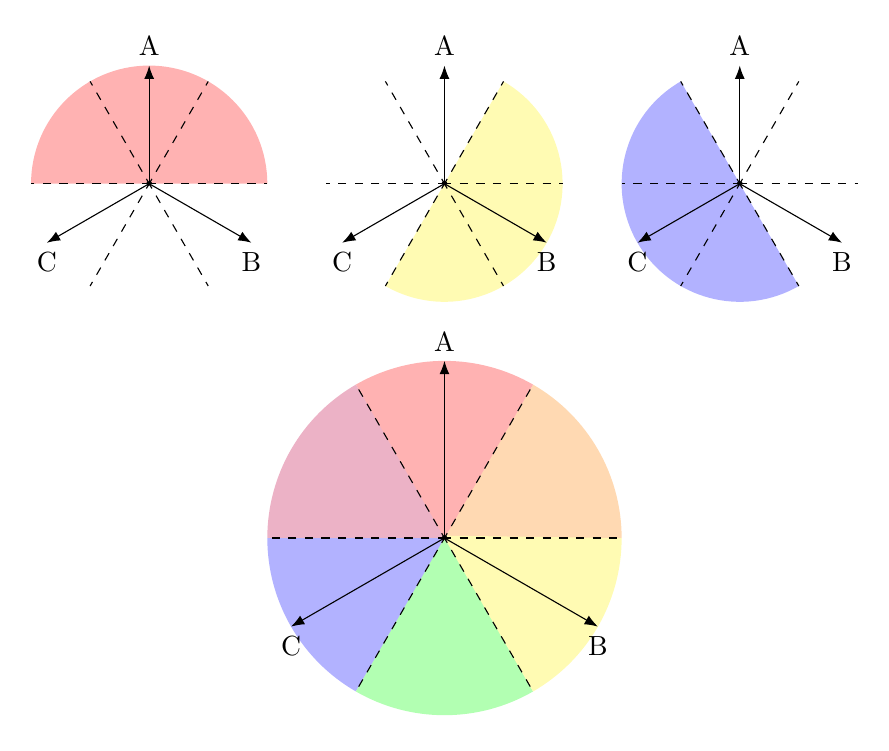
\begin{tikzpicture}[scale = 0.75,dummynode/.style={outer sep=-1,inner sep=-1}]
	\def\axe{2};
	\def\Baxe{3};
	\def\B{1};
	\def\xint{5};
	\def\yint{6};
	\def\tm{30};
	
	\draw (0,0)node[dummynode](OA){};
	\fill[red!\tm!white] (OA) -- ++(0:\axe)  arc[start angle = 0, end angle = 180,radius = \axe] -- cycle;
	\draw [-Latex] (OA) -- ++(90:\axe) node(A)[above]{A};
	\draw [-Latex] (OA) -- ++(-30:\axe) node(B)[below]{B};
	\draw [-Latex] (OA) -- ++(210:\axe) node(C)[below]{C};	
	\foreach \t in {0,60,...,300}
		\draw [dashed] (OA) -- ++(\t:\axe);
		
	\draw (0,0)++(\xint,0) node[dummynode](OB){};
	\fill[yellow!\tm!white] (OB) -- ++(-120:\axe)  arc[start angle = -120, end angle = 60,radius = \axe] -- cycle;
	\draw [-Latex] (OB) -- ++(90:\axe) node(A)[above]{A};
	\draw [-Latex] (OB) -- ++(-30:\axe) node(B)[below]{B};
	\draw [-Latex] (OB) -- ++(210:\axe) node(C)[below]{C};	
	\foreach \t in {0,60,...,300}
		\draw [dashed] (OB) -- ++(\t:\axe);
		
	\draw (OB)++(\xint,0) node[dummynode](OC){};
	\fill[blue!\tm!white] (OC) -- ++(120:\axe)  arc[start angle = 120, end angle = 300,radius = \axe] -- cycle;
	\draw [-Latex] (OC) -- ++(90:\axe) node(A)[above]{A};
	\draw [-Latex] (OC) -- ++(-30:\axe) node(B)[below]{B};
	\draw [-Latex] (OC) -- ++(210:\axe) node(C)[below]{C};	
	\foreach \t in {0,60,...,300}
	\draw [dashed] (OC) -- ++(\t:\axe);

	\draw (OB)++(0,-\yint) node[dummynode](O){};
	\fill[orange!\tm!white] (O) -- ++(0:\Baxe)  arc[start angle = 0, end angle = 60,radius = \Baxe] -- cycle;
	\fill[red!\tm!white] (O) -- ++(60:\Baxe)  arc[start angle = 60, end angle = 120,radius = \Baxe] -- cycle;
	\fill[purple!\tm!white] (O) -- ++(120:\Baxe)  arc[start angle = 120, end angle = 180,radius = \Baxe] -- cycle;
	\fill[blue!\tm!white] (O) -- ++(180:\Baxe)  arc[start angle = 180, end angle = 240,radius = \Baxe] -- cycle;
	\fill[green!\tm!white] (O) -- ++(240:\Baxe)  arc[start angle = 240, end angle = 300,radius = \Baxe] -- cycle;
	\fill[yellow!\tm!white] (O) -- ++(300:\Baxe)  arc[start angle = 300, end angle = 360,radius = \Baxe] -- cycle;
	\draw [-Latex] (O) -- ++(90:\Baxe) node(A)[above]{A};
	\draw [-Latex] (O) -- ++(-30:\Baxe) node(B)[below]{B};
	\draw [-Latex] (O) -- ++(210:\Baxe) node(C)[below]{C};	
	\foreach \t in {0,60,...,300}
		\draw [dashed] (O) -- ++(\t:\Baxe);
	
	\end{tikzpicture}
	\caption{通过霍尔传感器检测转子磁场位置}\label{figure:霍尔传感器检测转子磁场位置}
\end{figure}


\subsection{实验过程}
\subsubsection{线路连接}\label{sec:实验一线路连接}
\par
将电机A、B、C三相电源线与开发板上三组H桥的输出端子连接,将电机三条霍尔传感器输出线与开发板三个IO端口连接,再为开发板连接上直流电源线即完成了电气部分连接。
\par
此外,将开发板上的RJ45接口与仿真器连接,再将仿真器与计算机的USB口连接,即完成了调试通信部分连接。
\subsubsection{程序实现}
\paragraph{定子磁场的产生}
通过处理器的六路PWM波输出控制三组H桥上下桥臂的六个开关管即可实现对A、B、C三相电压的控制,从而实现定子绕组电流方向控制,产生每个时刻需要的定子磁场组合。\dsp 的PWM模块提供了OVDCON寄存器来方便使用者再不改变每路PWM输出的其他配置(如占空比)的情况下直接控制每路PWM信号的输出与否。
\begin{figure}[h]
	\centering
	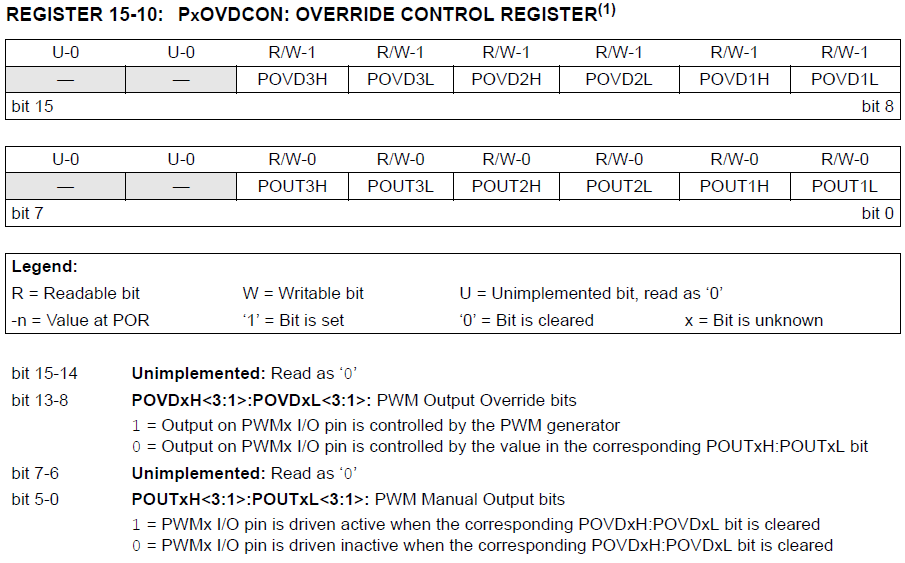
\includegraphics[scale=0.45]{OVDCON.png}
\end{figure}
\par
通过对寄存器中的第8-13位置1,可以使得对应的PWM正常输出,置0,则使得对应PWM的输出由该寄存器中第0-5位决定。因此,可以得到产生前述六种磁场与对应的OVDCON寄存器值之间的关系如表\ref{table:定子磁场与OVDCON关系}所示。(设PWM1对应A相,PWM2对应B相,PWM3对应C相)。
\begin{table}[h]
	\centering
	\caption{定子磁场与OVDCON寄存器的对应关系}\label{table:定子磁场与OVDCON关系}
	\begin{tabular}{>{\centering\arraybackslash}p{7em}>{\centering\arraybackslash}p{4em}>{\centering\arraybackslash}p{4em}>{\centering\arraybackslash}p{4em}>{\centering\arraybackslash}p{7em}}
		\toprule[1pt]
		定子磁场组合& PWM1&PWM2&PWM3&OVDCON值\\
		\midrule
		$A^{+}B^{-}$& H&L&0&0x0204\\
		$B^{-}C^{+}$& 0&L&H&0x2004\\
		$A^{-}C^{-}$& L&0&H&0x2001\\
		$A^{-}B^{+}$& L&H&0&0x0801\\
		$B^{+}C^{-}$& 0&H&L&0x0810\\
		$A^{+}C^{-}$& H&0&L&0x0210\\
		零磁场& 0&0&0& 0x0000\\
		\bottomrule[1pt]
	\end{tabular}
\end{table}

\paragraph{转子位置检测}
在任意时刻读取三路霍尔传感器的值即可得到该时刻转子磁场所在的扇区,再根据当前需要的旋转方向由图\ref{figure:扇区划分}和图\ref{figure:霍尔传感器检测转子磁场位置}选择需要的定子磁场组合,再根据表\ref{table:定子磁场与OVDCON关系}为OVDCON设置上相应的值即可完成电机运行的控制。在程序中,三相霍尔传感器的输入在寄存器中由高位到低位按照CAB的顺序依次排列,由此可得到控制电机旋转的逻辑关系如表\ref{table:霍尔传感器与PWM}所示。
\begin{table}[h]
	\centering
	\caption{霍尔传感器输入与PWM输出对应关系}\label{table:霍尔传感器与PWM}
	\begin{tabular}{>{\centering\arraybackslash}p{7em}p{3em}>{\centering\arraybackslash}p{10em}p{1em}>{\centering\arraybackslash}p{10em}p{0.5em}}
		\toprule[1pt]
		
		\begin{tabular}{>{\centering\arraybackslash}p{3em}>{\centering\arraybackslash}p{4em}}
			\multicolumn{2}{c}{霍尔传感器输入}\\
			\midrule
			CAB&十进制\\
			\midrule
			001&1\\
			010&2\\
			011&3\\
			100&4\\
			101&5\\
			110&6
		\end{tabular}& &
		\begin{tabular}{>{\centering\arraybackslash}p{4em}>{\centering\arraybackslash}p{5em}}
			\multicolumn{2}{c}{逆时针转动}\\
			\midrule
			定子磁场&OVDCON\\
			\midrule
			$A^{+}C^{-}$&0x0210\\
			$B^{-}C^{+}$&0x2004\\
			$A^{+}B^{-}$&0x0204\\
			$A^{-}B^{+}$&0x0801\\
			$B^{+}C^{-}$&0x0810\\
			$A^{-}C^{+}$&0x2001
		\end{tabular}& &
		\begin{tabular}{>{\centering\arraybackslash}p{4em}>{\centering\arraybackslash}p{5em}}
			\multicolumn{2}{c}{顺时针转动}\\
			\midrule
			定子磁场&OVDCON\\
			\midrule
			$A^{-}C^{+}$&0x2001\\
			$B^{+}C^{-}$&0x0810\\
			$A^{-}B^{+}$&0x0801\\
			$A^{+}B^{-}$&0x0204\\
			$B^{-}C^{+}$&0x2004\\
			$A^{+}C^{-}$&0x0210
		\end{tabular}& \\
		
		
		\bottomrule[1pt]
	\end{tabular}
\end{table}
\paragraph{转速的开环控制}
对于无刷直流电机,由于转子磁场由永磁体产生,因此只能通过调节定子磁场来改变力矩,从而改变转速。通过控制PWM波占空比能够改变每相的电流,也就能够改变转速。
\par
在开环控制实验中,以开发板上的电位器旋钮作为输入源,通过\dsp 的一路ADC采样得到电位器的分压值,等比例地设置为PWM波占空比,即完成了电机转速地开环控制。

\subsubsection{程序设计框图}
\paragraph{主程序}
主程序部分主要实现定时器、PWM、ADC、IO模块的初始化与设置工作,之后进入死循环维持程序运行,并通过一系列的循环判断来实现开发板上两个按钮外设对电机启停和转向的控制。程序流程框图如\ref{figure:实验一主程序流程图}所示。
\begin{figure}[h]
	\centering
	\begin{tikzpicture}[
	be/.style = {rectangle,minimum size = 6mm,rounded corners = 3mm,draw,inner xsep = 5pt,inner ysep = 5pt},
	do/.style = {rectangle,minimum size = 6mm,draw,align = center,inner xsep = 5pt,inner ysep = 5pt},
	ifl/.style = {shape aspect = 3,diamond,draw,label = -65:Y,label = 170:N,inner xsep = 5pt,inner ysep = 0pt},
	ifr/.style = {shape aspect = 3,diamond,draw,label = -115:Y,label = 10:N,inner xsep = 5pt,inner ysep = 0pt},]
	\draw (0,0) node(begin)[be]{进入主程序};
	\draw (begin)++(0,-1.25) node(init)[do]{模块初始化};
	\draw (init)++(0,-2) node(s21)[ifl]{S2按钮未按下};
	\draw (s21)++(0,-2.25) node(s31)[ifl]{S3按钮被按下};
	\draw (s31)++(0,-2.25) node(s32)[ifl]{S3按钮松开};
	\draw (s32)++(0,-1.75) node(direct)[do]{旋转方向标志位反转};
	\draw (direct)++(0,-2) node(s22)[ifl]{S2按钮被按下};
	\draw (s22)++(0,-2) node(settable)[do]{根据方向标志位\\ 和霍尔传感器值\\ 设置OVDCON};
	
	\draw (init)++(7,0) node(enPWM)[do]{使能PWM输出};
	\draw (enPWM)++(0,-1.25) node(setrunflag)[do]{运行标志位置高};
	\draw (setrunflag)++(0,-1.25) node(entimer)[do]{启动计时器};
	\draw (entimer)++(0,-2) node(ifrun)[ifr]{运行标志位=1?};
	\draw (ifrun)++(0,-2.25) node(s23)[ifr]{S2按钮被按下};
	\draw (s23)++(0,-1.75) node(stopPWM)[do]{关闭PWM输出};
	\draw (stopPWM)++(0,-1.25) node(deleterunflag)[do]{运行标志位清零};
	\draw (deleterunflag)++( 0,-2) node(s24)[ifr]{S2按钮被按下};
	
	\draw [-Latex] (begin.south) -- (init.north);
	\draw [-Latex] (init.south) -- (s21.north);
	\draw [-Latex] (s21.south) -- (s31.north);
	\draw [-Latex] (s21.west) -- ++(-0.75,0)node(L1){} |- ($0.5*(s21.north)+0.5*(init.south)$)node(T1){};
	\draw [-Latex] (s31.south) -- (s32.north);
	\draw [-Latex] (s31.west) -- (s31.west-|L1) |- ($(s31.north)!0.5!(s21.south)$);
	\draw [-Latex] (s32.south) -- (direct.north);
	\draw [-Latex] (s32.west) -- (s32.west-|L1) |- ($(s31.south)!0.5!(s32.north)$);
	\draw [-Latex] (direct.south) -- (s22.north);
	\draw [-Latex] (s22.south) -- (settable.north);
	\draw [-Latex] (s22.west) -- (s22.west-|L1) |- ($(s22.north)!0.5!(direct.south)$);
	
	\draw [-Latex] (settable.east) -| ($(init)!0.5!(enPWM)$) -- (enPWM.west);
	\draw [-Latex] (enPWM.south) -- (setrunflag.north);
	\draw [-Latex] (setrunflag.south) -- (entimer.north);
	\draw [-Latex] (entimer.south) -- (ifrun.north);
	\draw [-Latex] (ifrun.south) -- (s23.north);
	\draw [-Latex] (ifrun.east) -- ++(0.75,0)node(R1){} |- ($(ifrun.north)!0.5!(entimer.south)$);
	\draw [-Latex] (s23.south) -- (stopPWM.north);
	\draw [-Latex] (s23.east) -- (s23.east-|R1) |- ($(s23.north)!0.5!(ifrun.south)$);
	\draw [-Latex] (stopPWM.south) -- (deleterunflag.north);
	\draw [-Latex] (deleterunflag.south) -- (s24.north);
	\draw [-Latex] (s24.east) -- (s24.east-|R1) |- ($(s24.north)!0.5!(deleterunflag.south)$);
	\draw [-Latex] (s24.south)  |- ($(settable.south)+(0,-0.5)$)node(B1){} -| ($(L1)+(-1,0)$) |- (L1|-T1);
	
	\end{tikzpicture}
	\caption{实验一主程序流程图}\label{figure:实验一主程序流程图}
\end{figure}

\paragraph{ADC中断}
在开环控制中,将ADC采集到的电位器分压值乘上一定系数后直接作为PWM的占空比,从而实现对转速的开环调节。中断内流程框图如图\ref{figure:实验一ADC中断框图}所示。
\begin{figure}[h]
	\centering
	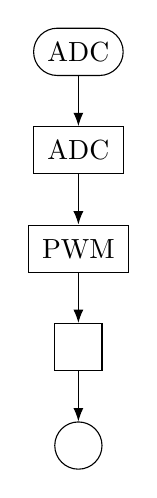
\begin{tikzpicture}[
	be/.style = {rectangle,minimum size = 6mm,rounded corners = 3mm,draw,align = center,inner xsep = 5pt,inner ysep = 5pt},
	do/.style = {rectangle,minimum size = 6mm,draw,align = center,inner xsep = 5pt,inner ysep = 5pt},
	ifl/.style = {shape aspect = 3,diamond,draw,label = -65:Y,label = 170:N,inner xsep = 5pt,inner ysep = 0pt},
	ifr/.style = {shape aspect = 3,diamond,draw,label = -115:Y,label = 10:N,inner xsep = 5pt,inner ysep = 0pt},]
	\def\hbb{1.25};
	\def\hbd{1.25};
	\def\hdd{1.25};
	\def\hbi{2};
	\def\hdi{2};
	\def\hii{2.25};
	\def\hib{1.75};
	\def\hid{1.75};
	
	\draw (0,0) node(begin)[be]{进入ADC中断};
	\draw (begin) ++(0,-\hbd)node(getADC)[do]{获取ADC采样值};
	\draw (getADC) ++(0,-\hdd)node(setduty)[do]{设置PWM占空比};
	\draw (setduty) ++(0,-\hdd) node(clearintflag)[do]{清除中断标志位};
	\draw (clearintflag) ++(0,-\hbd) node(exit)[be]{退出中断};
	
	\foreach \x/\y in {begin/getADC,getADC/setduty,setduty/clearintflag,clearintflag/exit}
		\draw [-Latex] (\x.south) -- (\y.north);
	
	\end{tikzpicture}
	\caption{实验一ADC中断框图}\label{figure:实验一ADC中断框图}
\end{figure}
\subsubsection{代码清单及注释}
\paragraph{SensoredBLDC.c}
\paragraph{Interrupts.c}
\paragraph{Init.c}

\section{BLDC闭环控制}
\subsection{实验目标}
\begin{enumerate}[a.,topsep=0pt]
	\setlength{\itemsep}{-0.25\baselineskip}
	\item 在实验一实现的BLDC启动、运行的基础上,增加转速的闭环控制。
	\item 通过霍尔传感器的输出实现BLDC的转速测定。
	\item 通过开发板上的电位器旋钮作为输入,实现对BLDC转速的精确给定。
\end{enumerate}
\subsection{实验原理}
\subsubsection{转速闭环PI控制}
\par
根据自动控制原理课程的知识可知,为了使实际转速$n$与给定转速$n^{*}$相同,需要引入反馈环节,将两者比较后的结果作为控制系统的输入量,直到速度差$\Delta n = 0$。
\par
而为了实现无差调节,往往采用PI控制方式,控制系统的框图如图\ref{figure:实验二BLDC闭环控制框图}所示。
\begin{figure}[h]
	\centering
	\begin{tikzpicture}[
	sum/.pic = {
		\coordinate (-north) at (0,0.2);
		\coordinate (-east) at (0.2,0);
		\coordinate (-south) at (0,-0.2);
		\coordinate (-west) at (-0.2,0);
		\coordinate (-o) at (0,0);		
		\draw (0,0) circle [radius = 0.2];
		\draw (-north) -- (-south);
		\draw (-east) -- (-west);},
	p/.style = {rectangle,minimum size = 6mm,draw,align = center,inner xsep = 5pt,inner ysep = 5pt},
	ifl/.style = {shape aspect = 3,diamond,draw,label = -65:Y,label = 170:N,inner xsep = 5pt,inner ysep = 0pt},
	ifr/.style = {shape aspect = 3,diamond,draw,label = -115:Y,label = 10:N,inner xsep = 5pt,inner ysep = 0pt},]
	\def\hbb{1.25};
	\def\hbd{1.25};
	\def\hdd{1.25};
	\def\hbi{2};
	\def\hdi{2};
	\def\hii{2.25};
	\def\hib{1.75};
	\def\hid{1.75};
	
	\pic (sum1) at (0,0) {sum};
	\draw (sum1-o)++(4,0) node(KP)[p]{$K_P$} ++ (0,1.5) node(KI)[p]{$\frac{K_I}{s}$};
	\draw (KP)++(2,0) pic (sum2){sum} ++(3,0) node(Ks)[p]{$H_{m}\left(s\right)$};
	
	\draw [-Latex] (sum1-west)++(-2,0) -- (sum1-west) node[pos=0.5,above]{$n^{*}$} node[pos=0.9,above]{$+$}; 
	\draw [-Latex] (sum1-east) -- (KP.west) node[pos = 0.25,above]{$\Delta n$};
	\draw [-Latex] ($(sum1-east)!0.5!(KP.west)$) |- (KI.west);
	\draw [-Latex] (KP.east) -- (sum2-west);
	\draw [-Latex] (KI.east) -| (sum2-north);
	\draw [-Latex] (sum2-east) -- (Ks.west) node[pos=0.5,above]{$D$};
	\draw [-Latex] (Ks.east) -- ++(2,0) node(out)[pos=0.5,above]{$n$};
	\draw [-Latex] (out) -- ++(0,-1.5) -| (sum1-south) node[pos=0.9,left]{$-$};
	
	\end{tikzpicture}
	\caption{BLDC闭环控制框图}\label{figure:实验二BLDC闭环控制框图}
\end{figure}
\par
图中,$K_P$为PI环节的比例调节系数,$K_I$为PI环节的积分调节系数,$D$为占空比输出,$H_{m}\left(s\right)$为H桥及电机的传递函数。
\par
为了达到稳定状态,要求控制系统输出的占空比应为一常数,又由于积分环节$\sfrac{K_{I}}{s}$的存在,只有到积分环节输入$\Delta n = 0$时,积分输出才不再变化,因此,采用PI调节能够实现电机转速的无静差调节。而通过调节比例系数$K_P$和积分系数$K_I$,能够调整控制系统的动态相应特性,如调整时间、最大超调量等。

\paragraph{电机速度测定}
能够实现闭环PI调节的前提是能够准确测定电机实际转速,从而形成反馈。由于已经有安装在电机内的霍尔传感器能够获取电机转子的角度位置信息,只需要配合\dsp 处理器内部的定时器模块,测定转子磁场进入图\ref{figure:霍尔传感器检测转子磁场位置}中某一扇区的时间间隔$\Delta t$,在已知电机极对数的情况下,既可以计算得到电机实际转速:
\begin{shrinkeq}{-1.5ex}{-2.5ex}
	\begin{align}
	n = \frac{60}{p\Delta t}
	\end{align}
\end{shrinkeq}
\subsection{实验过程}
\subsubsection{线路连接}
\par
本次实验线路连接与实验一(\ref{sec:实验一线路连接})相同,这里不再赘述。
\subsubsection{程序实现}
\paragraph{转速测定}

\end{spacing}


	
\end{document}